\subsection{Принцип работы}

На данном микроконтролере существует 6 различных портов:
\begin{itemize}
    \item GPIOA
    \item GPIOB
    \item GPIOC
    \item GPIOD
    \item GPIOE
    \item GPIOF
\end{itemize}   

У каждого порта по 16 пинов. Однако в большинстве случаем в виду органиченности ножек микроконтролера не все порты реализуются полностью. В случае нашей платы: три пинат заняты под два стедиода и одну кнопку, два пина заняты для соединения с программатором. 


Управление с пинами осуществляем с помощью LL функцией.

\begin{verbatim}
    //обычная функция для записи в регистр
    LL_GPIO_SetPinMode(GPIOx, LL_GPIO_PIN_x, Regime) ;
    //За один раз данная функция фонкфигурирует только один пин.

    //Настройка тип цифрового выхода
    LL_GPIO_SetPinOutputMode(GPIOx, LL_GPIO_PIN_x, Regime);
    // Аналогично только один пин.
    
    //Функции для изменения выходного состояния
    LL_GPIO_WriteOutputPort(GPIOx, output_value); -> ODR
    
    LL_GPIO_WriteOutputPin(GPIOx, bits_of_pins); -> BSRR
    
    LL_GPIO_ResetOutputPin(GPIOx, bits_of_pins); -> BRR
    //Можно писать в несколько пинов!
    

\end{verbatim}


\subsection{Дребезг контактов}


\begin{figure}[h!]
		\centering
		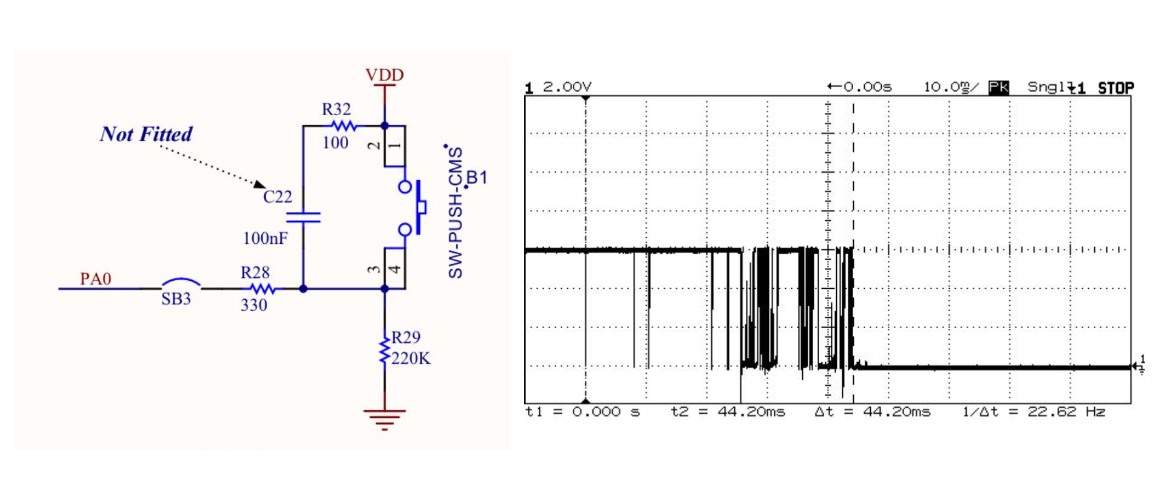
\includegraphics[width=1\linewidth]{pics/drebezg.png}
		\caption{Устройства подключения кнопки и график с дребезгом}
		\label{drebezg}
\end{figure}

На картинке \ref{drebezg} показано подключение кнопки $USER$ на нашей отладочной плате. 
	
	
\begin{figure}[h!]
		\centering
		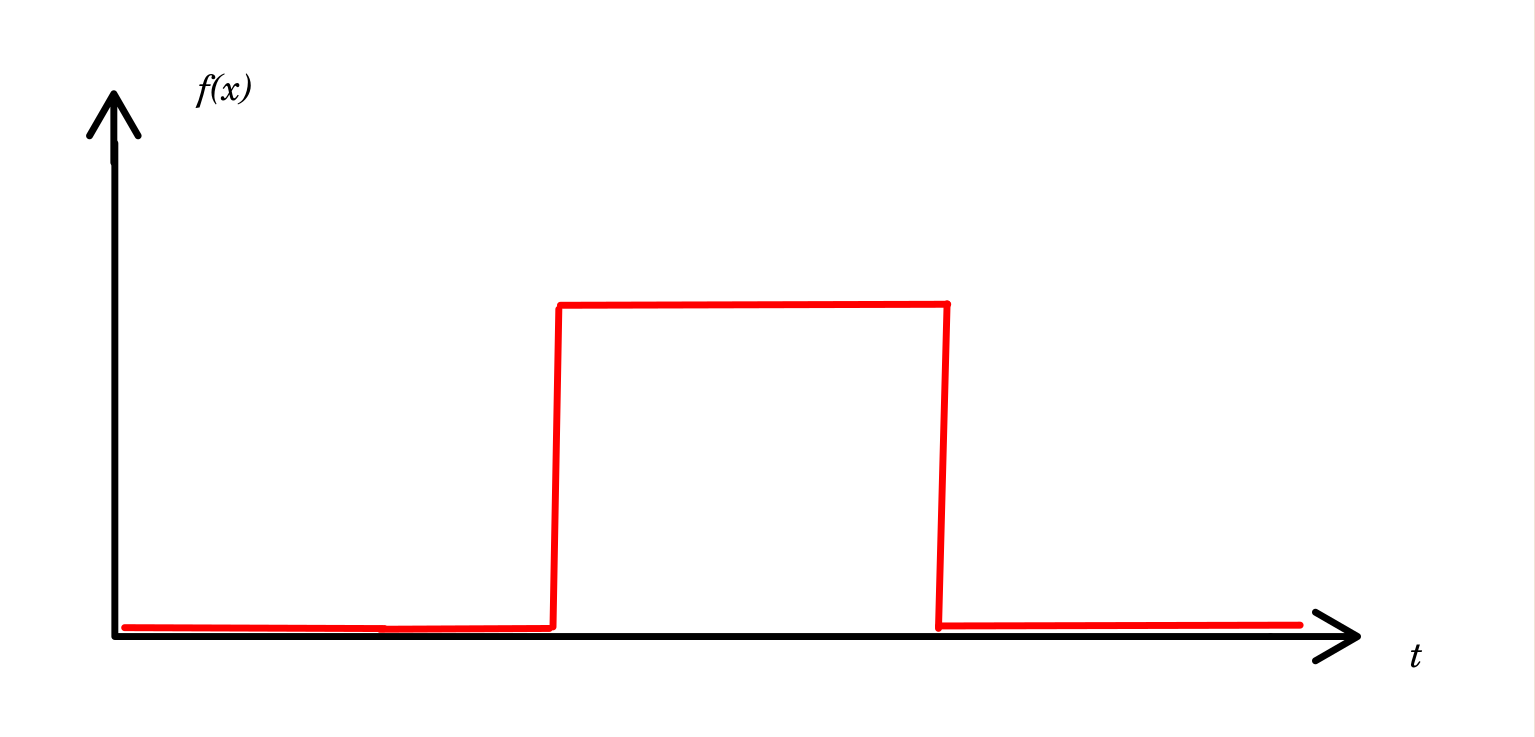
\includegraphics[width=1\linewidth]{pics/ideal_sing.png}
		\caption{Идеальный график сигнала}
		\label{drebezg}
\end{figure}
	
Проблема дребезга 

